\chapter{基础知识}
\label{ch2}
在本章节中我们将介了本文研究所需要的一些基本知识,有助于更好的理解之后章节的内容。

\section{联邦学习}

\subsection{基本概念}
深度学习的成功应用需要建立在大量数据的基础之上,才能完成人们指派的学习任务。然而,近年来数据泄漏和隐私侵权事件不断发生,用户开始更加关注他们的隐私信息是否未经自己的许可,或被他人出于商业或者政治目的而被利用。人们逐渐地意识到,在人工智能的构建与使用的过程中保护用户隐私和数据机密的重要性。

大部分拥有的训练数据是由不同组织的个人、部门产生并拥有的,传统机器学习的做法是收集数据并传输到一个中心服务器,服务器可以看见并控制所有的数据,因此这个中心点不仅需要拥有高性能的计算集群来训练和建立机器学习模型,而且还需要处理敏感数据,避免泄漏用户隐私。然而,这种方法需要用户对服务器的完全信任,这已经不再有效或适用了。在这样的情况下,数据拥有者倾向于将自己的数据保留在自己的手中,进而会形成各自孤立的数据孤岛,至此大量数据的基础已经消失,人工智能的未来将面临绝境。作为回应,2016 年谷歌\upcite{ref25}率先提出联邦学习概念,旨在建立高质量分布式学习的框架。在联邦学习系统中,数据所有者(参与者)不需要彼此共享原始数据,也不需要依赖单个可信实体(中心服务器)来进行机器学习模型的分布式训练。相反,参与者通过在自己的本地数据上执行本地训练算法,并且只与参数服务器共享模型参数,来共同协作训练联邦模型。在每轮训练中,参数聚合节点会随机选择合适的节点加入到训练池中。那些被选中的本地节点通常是保持充电且无线网络可用。然后参数聚合节点平均所有已提交者的权重并作为下一轮回合的初始化模型。重复此过程直至终止条件。

\subsection{联邦学习的分类}

根据用户维度和模型特征维度的重合去分类,将联合学习分为水平联邦学习、纵向联邦学习和联合迁移学习\upcite{ref26}。
\begin{itemize}
\item \textbf{水平联邦学习}:当两个数据集的用户属性重叠较多而用户重叠较少的情况下,我们对数据集进行横向切割(即按用户维度切割),取出两边用户属性相同但用户不完全相同的那部分数据用于训练。这种方法被称为横向联合学习。例如,两家银行位于不同的地区,有来自各自地区的用户群,而且它们之间的联系非常少。然而,他们的业务活动非常相似,因此他们的用户特征也是一样的。在这个阶段,我们可以使用跨部门的联邦学习来建立一个联合模型。2016年,谷歌提出了一个在安卓手机上更新模型的联合数据建模系统:模型参数在本地不断更新,并在各个用户使用安卓手机时上传到安卓云端,使拥有数据的每一方都能建立一个具有相同特征维度的联合模型。

\item \textbf{纵向联邦学习}:在两个数据集中用户重叠较多,而用户属性重叠较少的情况下,我们将数据集纵向切开(即按特征维度),选择数据集中两边用户相同但用户属性不完全相同的部分进行训练。这种方法被称为纵向的联邦学习。例如,有两个不同的组织,一个是在一个地方的银行,另一个是在同一个地方的电子商务公司。他们的用户群很可能包括该地的大部分人口,所以有很大的用户交集。然而,由于银行储存的是用户的收入和支出以及信用评分的数据,而电子商务公司储存的是用户的浏览和购买历史的数据,他们的用户档案并没有那么紧密的联系。纵向的联邦学习是在一个加密的空间里将这些不同的功能结合起来,以提高模型的性能。

\item \textbf{联合迁移学习}:联合迁移学习是通过使用迁移学习模型来弥补数据或标签的差距,而不是对数据进行切分。当两个数据集中的用户和用户属性几乎没有重叠。这种方法被称为联合迁移学习。这里举一个例子,考虑两个不同的组织,一个是中国的银行,另一个是美国的电子商务公司。由于地理上的限制,这两个机构的用户群重叠的地方很少。由于它们是不同类型的组织,数据的特点也没有太多的重叠。在这种情况下,为了保证有效的联邦学习,可以引入联合迁移学习,以克服单变量数据量小和标注样本小的问题,提高模型的效率。

\end{itemize}

\subsection{模型框架}

\begin{figure}[!hbt]
\centering
	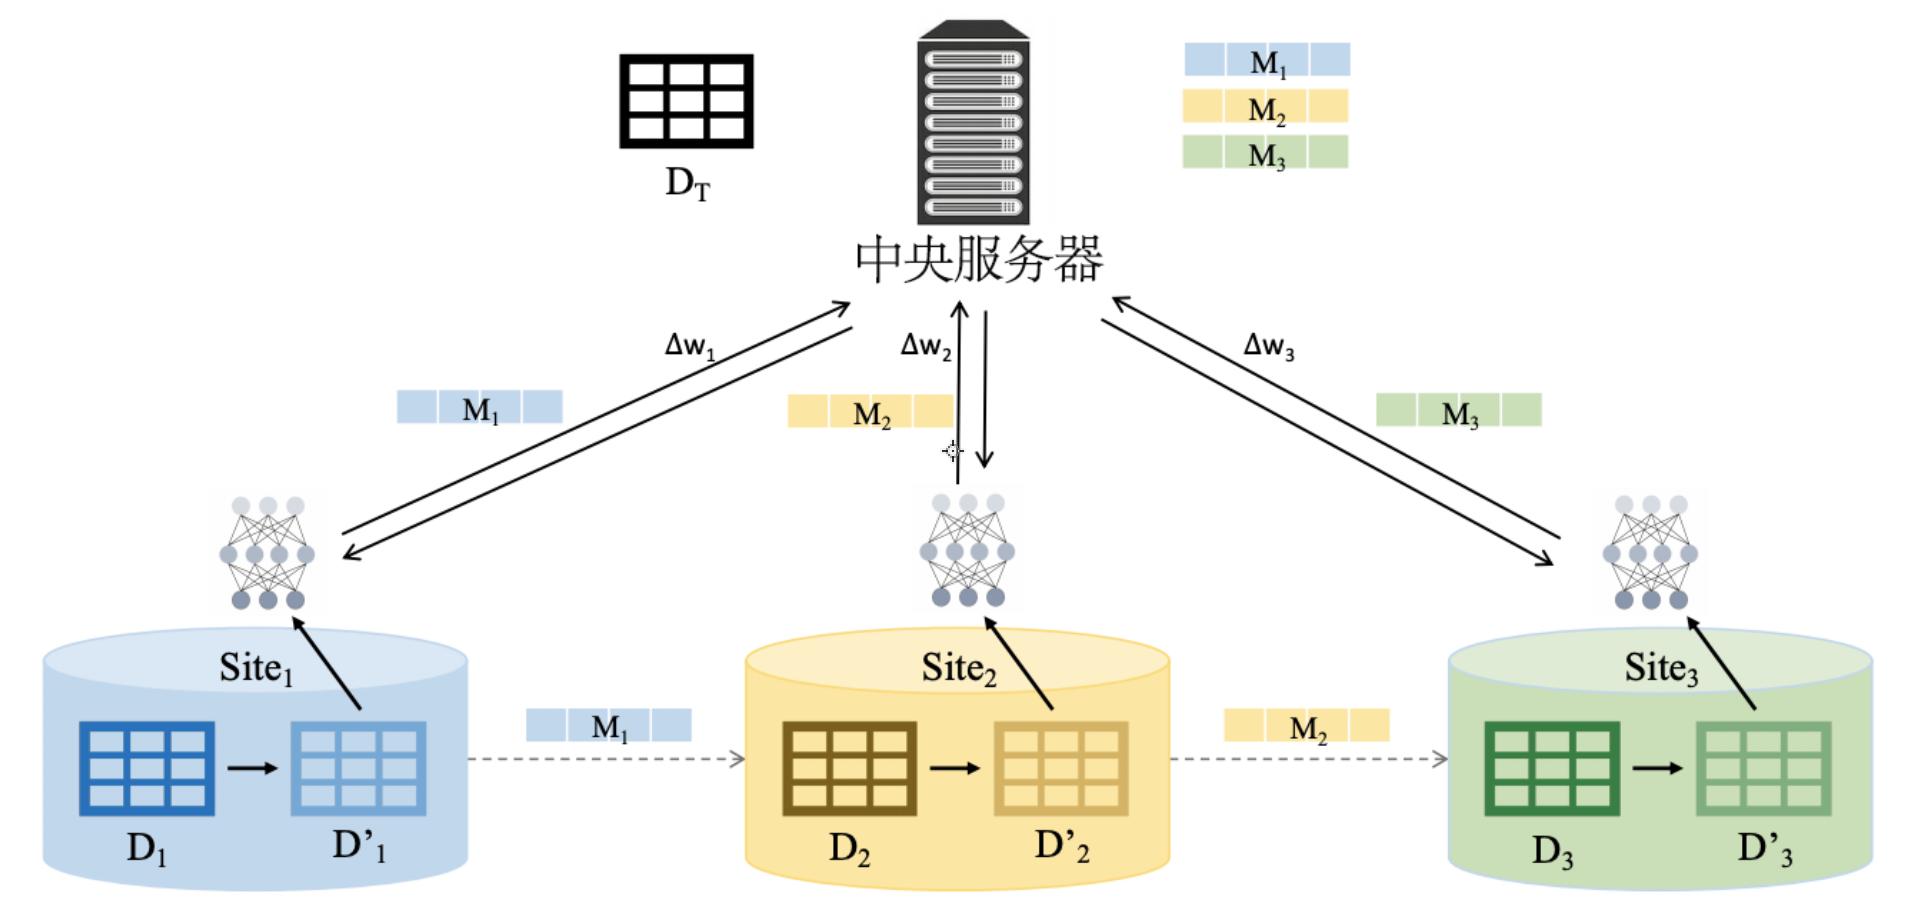
\includegraphics[scale=0.45]{fig2/C2/联邦学习模型流程}%联邦学习的系统架构
	\caption{联邦学习模型工作流程}
	\label{fig:联邦学习模型工作流程}	
\end{figure}

本文我们提出的方案是基于典型的分布式横向联邦学习系统架构,即各个参与者的本地数据集特征空间相同,但样本不同。通过中心服务器,各个参与者相互协作,在保护个人本地敏感数据的同时,有效地提高本地学习效果。如图\ref{fig:联邦学习模型工作流程}所示,分布式横向联邦学习的基本工作流程如下:
\begin{itemize}
\item \textbf{初始化:}所有用户在他们的设备上都有一个预先分配的神经网络模型,并且可以自愿加入联邦学习协议,指定相同的深度学习和模型训练目标。
\item  \textbf{本地训练:}在一个给定的通信回合中,联邦学习参与者首先从中央服务器下载全局模型参数,然后使用他们的私人训练模式训练模型,更新本地模型(即模型参数),并将这些更新发送到中央服务器。
\item \textbf{中央参数聚合:}中央服务器汇总此次通信回合中所有参与者上传的模型参数,并对其进行聚合求得全局模型的参数,然后更新全局模型。
\item \textbf{迭代更新:}迭代地执行上述步骤直至全局模型参数满足收敛条件,最终得到最优的全局模型。
\end{itemize}{}

\section{深度神经网络}
\subsection{基本结构}
神经网络\upcite{ref34}的设计来源于人脑的结构,是人脑处理信息方式的一个简化模型。人类的大脑是人中枢神经系统中的主要部分,这些神经元像网状物一样相互连接。来自外部环境的刺激或来自感觉器官的输入通过感受器之后进入传入神经,神经元一层一层兴奋(激活)后,传导到神经中枢(大脑或脊髓),神经中枢(相当于输出层)根据信号的类型做出不同的判断(分类),然后再下达命令,将信号传递到输出神经。不同的信号,大脑都可以进行学习和分辨,而这一通用的模型,就是神经网络。

神经网络的基本单元是神经元,由数百万个简单的神经元组成,这些神经元密集地相互连接,神经元按层排列。每一层有多个神经元,层与层之间是"前馈传播"的,也就是说,网络中的数据只在一个方向上移动。一个单独的神经元可能与它前面一层的几个神经元相连,它从这些神经元接收数据;与它后面一层的几个神经元相连,它向这些神经元发送数据。神经元之间不存在同层连接,也不存在跨层连接。

\begin{figure}[!hbt]
\centering
	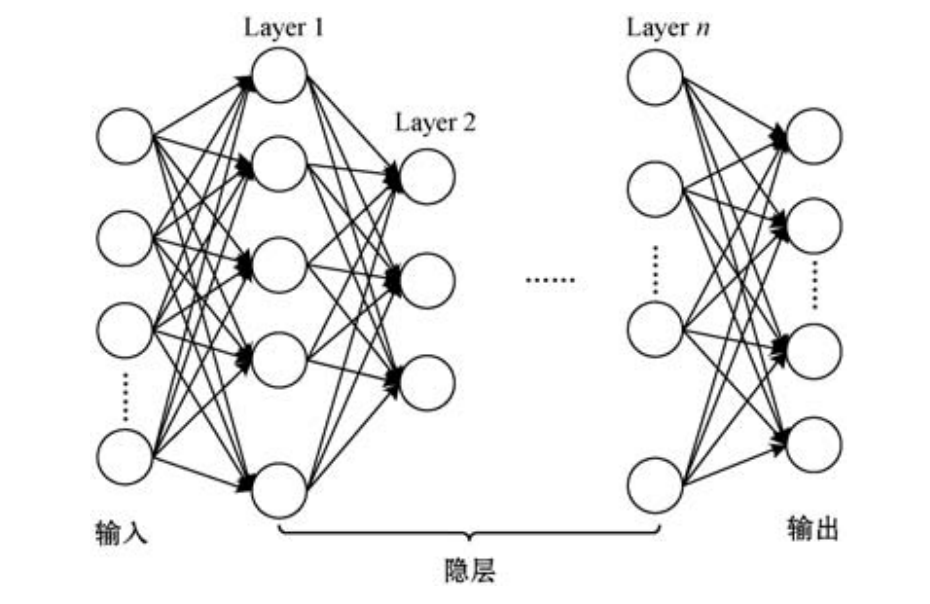
\includegraphics[scale=0.5]{fig2/C2/深度神经网络结构图}%联邦学习的系统架构
	\caption{深度神经网络结构图}
	\label{fig:深度神经网络结构图}	
\end{figure}

如图\ref{fig:深度神经网络结构图}所示,神经网络通常有三个部分:一个输入层,主要用于获取输入的信息;一个或多个隐藏层,主要进行特征提取,调整权重让隐藏层的神经单元对某种模式形成反应;以及一个输出层,对接隐藏层并输出模型结果,调整权重以对不同的隐藏层神经元刺激形成正确的反应。
当一个神经网络被训练时,其所有的权重和阈值最初都被设置为随机值。训练数据被送入输入层,并通过后续隐藏层,以复杂的方式相乘和相加,直到最后到达输出层,从根本上改变了数据。在训练过程中,不断调整网络的权重和阈值,直到具有相同标签的训练数据持续产生类似的输出。

\subsection{前向传播算法}

神经网络中层与层之间的” 前馈传播” 的算法简称为前向传播算法:网络中上一层的输出作为下一层的输入,并计算下一层的输出,一直到运算到输出层为止。如图\ref{fig:前馈神经网络结构图}所示,假设现有输入层的训练数据为$D=\left\{\left(x_{1}, y_{1}\right),\left(x_{2}, y_{2}\right), \cdots,\left(x_{m}, y_{m}\right)\right\}, x_{i} \in R^{d}, y_{i} \in R^{l}$,即输入样本由 $d$ 个属性描述, 输出是 $l$ 维实值向量。

\begin{figure}[!hbt]
\centering
	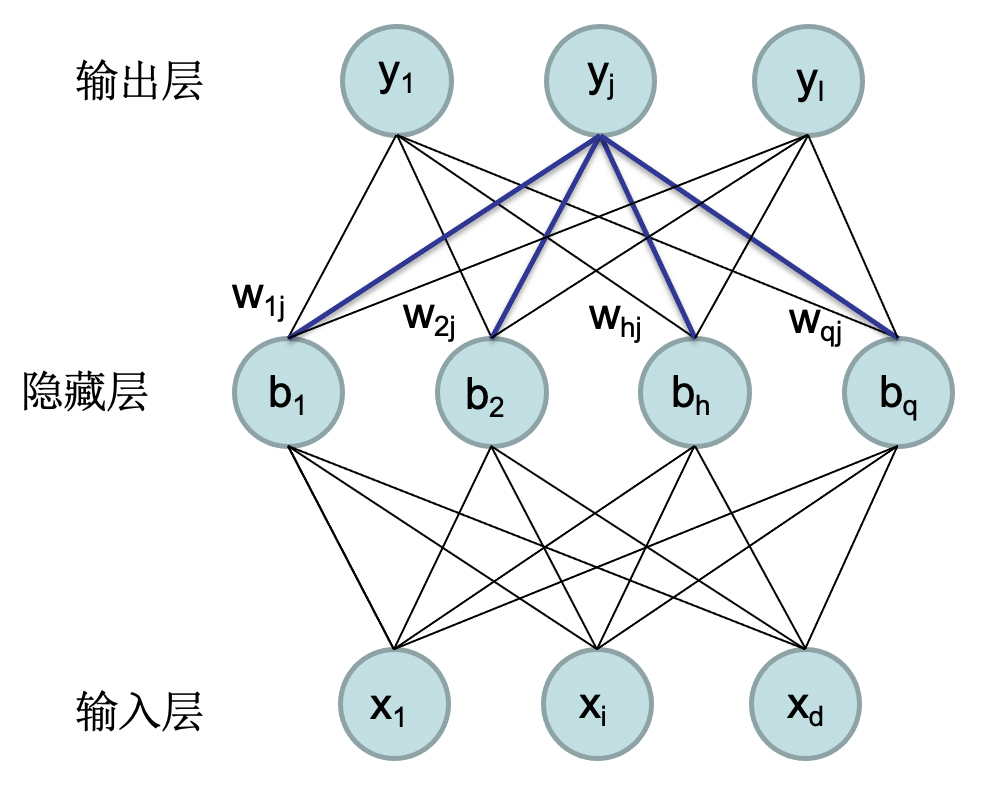
\includegraphics[scale=0.5]{fig2/C2/前馈神经网络}%
	\caption{前馈神经网络结构图}
	\label{fig:前馈神经网络结构图}	
\end{figure}

假设隐藏层神经元个数为$q$个,$\theta_{j}$ 表示输出层神经元的阈值。隐藏层第 $h$ 个神经元的阈值用 $\gamma_{h}$ 表示。
输入层第 $i$ 个神经元与隐藏层第 $h$ 个神经元之间的连接权为 $v_{i h}$。隐藏层第 $h$ 个神经元与输出层第$j$个神经元之间的连接权为 $w_{h j}$ 。
隐藏层第 $h$ 个神经元接收到的输入为$\alpha_{h}=\sum_{i=1}^{d} v_{i h} x_{i}$,输出层第$j$个神经元接收到的输入为$\beta_{j}=\sum_{h=1}^{q} w_{h j} b_{h}$。其中 $b_{n}$ 为隐藏层层第$h$ 个神经元的输 出。
假设隐层和输出层神经元都使用Sigmoid激活函数。对训练数据 $\left(x_{k}, y_{k}\right)$, 假定神经网络的输出为 $\hat{y}_{k}=\left(\hat{y}_{1}^{k}, \hat{y}_{2}^{k}, \cdots, \hat{y}_{l}^{k}\right)$, 即神经网络的预测输出表达式为:
\begin{equation}\label{神经网络预测输出}
\hat{y}_{j}^{k}=f\left(\beta_{j}-\theta_{j}\right)
\end{equation}

那么如何评估神经网络输出的预测值与真实值之间的差异程度呢?这里提出损失函数 $L$,本文采用均方差损失函数,这种损失是通过计算实际(目标)值和预测值之间的平方差的平均值,网络在样本集 $\left(x_{k}, y_{k}\right)$上的均方误差为:
\begin{equation}\label{神经网络损失函数}
E_{k}=\frac{1}{2} \sum_{j=1}^{l}\left(\hat{y}_{j}^{k}-y_{j}^{k}\right)^{2}
\end{equation}

\subsection{反向传播算法}
深度神经网络算法训练的目的就是使得损失函数 $L$ 最小,通常采用随机梯度下降(Stochastic Gradient Descent, SGD)算法,即在每次迭代过程中批量随机抽取训练样本 ($B$),并计算损失函数 $L$ 的偏导数 $g_{B}=\frac{1}{|B|} \sum_{x \in B} \nabla_{\theta} L(\theta,$,$x$ ),然后沿着负梯度方向 $-g_{B}$ 朝着局部最小值更新权重系数 $\theta_{\circ}$。
反向传播算法\upcite{ref29}基于梯度下降(gradient descent)\upcite{ref30}策略,依据输出层的输出结果计算误差,再将误差反向传播到隐藏层神经元,最后依据隐层神经元的误差来对连接权和阈值进行调整\upcite{ref31}。

总的来说,在深度神经网络中,对每个训练样本,通过前向传播算法从输入层、隐藏层到输出层依次训练,在输出层得到预测的结果,然后根据损失函数计算预测值与真实值之间的差异程度,之后根据反向传播算法调整权重系数,更新网络参数,使得损失函数的值最小,模型达到全局最优。

\section{差分隐私}
差分隐私最初是由微软研究院在2006年\upcite{ref9}针对统计数据库的隐私泄露问题提出的一种新的隐私定义,目的是使得数据库查询结果对于数据集中单个记录的变化不敏感。简单来说,就是单个记录在或者不在数据集中,对于查询结果的影响微乎其微。那么攻击者就无法通过加入或减少一个记录,观察查询结果的变化来推测个体的具体信息。

差分隐私首先被应用于数据查询,为了更好地说明数据集之间的差异,定义了相邻数据集的概念:两个数据集只差一个信息或只差一个数值不同的记录\upcite{ref28}。因此,查询数据库相关信息的攻击者将无法以任何概率确定$X_{n}$是否存在于数据集中,而成员$X_{n}$被认为是相对安全的。

\subsection{基本定义}
\begin{define}[邻近数据集]\label{邻近数据集}
现有数据集 $D$ 和 $D^{\prime}$,两者具有相同的属性结构,他们的对称差为$D \Delta D^{\prime},\left|D \Delta D^{\prime}\right|$ 表示 $D \Delta D^{\prime}$ 中记录的数量。若 $\left|D \Delta D^{\prime}\right|=1$,那么$D$ 和 $D^{\prime}$ 就是邻近数据集 (Adjacent Dataset)。
\end{define}

\begin{figure}[!hbt]
\centering
	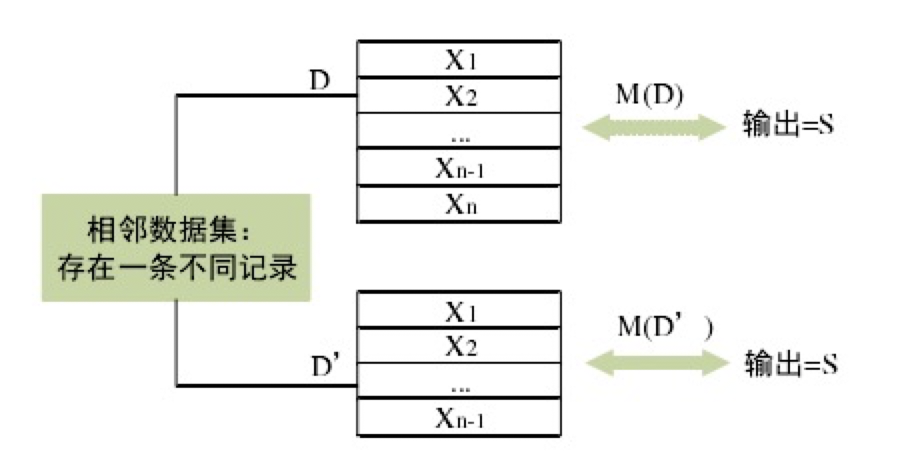
\includegraphics[scale=0.6]{fig2/C2/相邻数据集示意图}%联邦学习的系统架构
	\caption{差分隐私的相邻数据集示意图}
	\label{fig:相邻数据集示意图}	
\end{figure}

假设存在有限域 $Z,z \in Z$ 为 $Z$ 中的元素,从有限域 $Z$ 中抽样所得 $z$ 组成数据集 $D$,数据的属性个数为维度 $d$,样本量为$n$。对数据集 $D$ 的查询即映射函数,用 $F=\left\{f_{1}, f_{2}, \cdots\right\}$ 来表示一组查询,算法 $M$ 表示满足差分隐私的查询机制,它通过对查询 $F$ 的结果进行处理,使之满足隐私保护的条件。

\begin{define}[差分隐私成立条件]\label{差分隐私成立条件}

若随机算法 $M: D \rightarrow R$ 满足 $(\varepsilon, \delta)-D P$,当且仅当相邻数据集 $d, d^{\prime}$ 对于算法 $M$ 的所有可能输出子集 $S \in R$ 满足不等式 $^{[40]}$ :
$$
\operatorname{Pr}[M(d) \in S] \leq e^{\varepsilon} \operatorname{Pr}\left[M\left(d^{\prime}\right) \in S\right]+\delta
$$
\end{define}
其中,$\varepsilon$ 表示隐私预算参数,$\varepsilon$ 越接近0代表着数据集$D$,$D^{\prime}$ 上输出的数据分布越接近,输出结果越不可区分,隐私预算越低,隐私保护的强度越高。添加值$\delta$代表允许以概率 $\delta$ 打破 $\varepsilon-\mathrm{DP}$ 的可能性,是用于限制模型行为任意改变的概率,值通常选择小于 $1 /|D|$。当 $\delta=0$ 时,定义转化为 $\varepsilon-\mathrm{DP}$,这时机制提供了更加严格的隐私保护。隐私保护强度取决于隐私预算参数,在传统的数据保护领域,如果$\varepsilon \in(0,1)$,那么此时隐私保护强度是有用的,但是在深度学习方面,当$\varepsilon \in(0,10)$是才认为隐私保护强度是有效的。


\subsection{相关概念}
差分隐私保护的实现是在查询函数的返回值中注入一定量的干扰噪声,但是注入的噪声量太大会影响最终结果的准确性,太少则无法保障数据的隐私性。那么如何衡量添加的噪声量,既能保障数据的安全,又能维持数据的可用性呢?这里针对数据集提出敏感度的概念,加入的噪声量大小与数据集的敏感度息息相关。

对于数据集D,它的敏感度是指在数据集D中任意删除一条记录,对最终的查询结果产生的最大影响。数据集的敏感度决定了注入噪声量的大小。在差分隐私中有两种敏感度,分别是全局敏感度和局部敏感度。

\begin{define}[全局敏感度]\label{全局敏感度}
假设存在函数 $f: D \rightarrow R^{d}$, 输入为一数据集,输出为$d$维的实数向量。 对于任意的邻近数据集 $D$ 和 $D^{\prime}$,
$$
G S_{f}=\max _{D, D^{\prime}}\left\|f(D)-f\left(D^{\prime}\right)\right\|_{1}
$$
称为函数 $f$ 的全局敏感度。
\end{define}

全局敏感度由函数本身决定,反映了一个查询函数在一对相邻数据集上进行查询时变化的最大范围,它取决于查询函数本身,与数据集无关。
不同的函数会有不同的全局敏感度。但是如果全局敏感度太大,根据全局敏感度生成的噪声可能会过度保护数据,因此提出了局部敏感性的定义。

\begin{define}[局部敏感度]\label{局部敏感度}
对于一个查询函数 $f_{:} D \rightarrow R^{d}$, 其中 $D$ 为一个数据集, $R^{d}$为d维实数向量,是查询的返回结果。假使给定数据集D,它有任意邻近数据集 $D^{\prime}$, 查询函数$f$在$D$ 上的局部敏感度定义为:
$L S_{f}(D)=\max _{D^{\prime}}\left\|f(D)-f\left(D^{\prime}\right)\right\|_{1}$。
\end{define}

与全局敏感度不同,局部敏感度是由给定的数据集和查询函数共同决定的。由于局部敏感度只是对于一个数据集做变化,利用了数据集的数据分布特征,局部敏感度通常要比全局敏感度小得多。但是,也正是因为局部敏感度在某种程度上反映了数据集的分布特征,所以直接应用局部敏感度生成噪声可能会泄漏数据的隐私信息。

敏感度代表了查询函数针对相邻数据集的输出的最大不同,或者说量化评估了最坏情况下单个样本对整体数据带来的不确定性大小。敏感度函数仅与查询函数的类型有关,给噪声的添加提供了依据。

在解决一个复杂的差分隐私保护问题时,可能在多个场景,多个步骤多次应用差分隐私技术,在这种情况下,如何保证最终结果的差分隐私性,以及隐私保护的程度该如何去度量呢?这里引出差分隐私的三个最重要的性质:可量化性、可组合性和后处理不变性\upcite{ref35}。

可量化性指的是差分隐私算法在计算特定随机化过程时,可以透明化、精准量化所施加的噪声大小,即上文提及的隐私预算。这样使用者就可以清楚地知道算法的隐私保护力度;差分隐私的后处理不变性,确保了即使对算法的结果进行进一步处理,只要不引入额外信息,后续的处理就并不会削弱算法的隐私保护力度。组合性是指将相互独立的差分隐私算法进行组合\upcite{ref41}后依然满足差分隐私,具体可分为并行组合和串行组合。

\begin{theorem}[串行组合]\label{串行组合}
给定 $\mathbf{n}$ 个随机算法 $M_{i}(1 \leq i \leq n)$ 满足 $\varepsilon_{i}-DP$, 那么针对一个数据库 $D$ 而言, 在 $\mathrm{D}$ 上的算法串行序列组合满足$\varepsilon-\mathrm{DP}$, 其中 $\sum_{i=1}^{n} \varepsilon_{i}=\varepsilon$ 。
\end{theorem}

\begin{theorem}[并行组合]\label{并行组合}
如果数据库 $\mathrm{D}$, 划分成 $\mathrm{n}$ 个不相交的子集 $\left\{\mathrm{D}_{1}, \mathrm{D}_{2}, \ldots, \mathrm{D}_{n}\right\}$, 在每个子集上应用算法 $\mathrm{M}_{i}$, 每个算法提供 $\varepsilon_{i}-\mathrm{DP}$ , 则在序列 $\left\{\mathrm{D}_{1}, \mathrm{D}_{2}, \ldots, \mathrm{D}_{n}\right\}$ 上整体满足 $\left(\max \left\{\varepsilon_{1}, \ldots, \varepsilon_{n}\right\}\right)-\mathrm{DP}$。
\end{theorem}

通过差分隐私的串并行组合定理,人们可以利用基础的差分隐私算法设计出复杂的满足差分隐私保证的系统,只要算法中的每一个步骤都满足差分隐私要求,那么这个算法的最终结果将满足差分隐私特性,这也是差分隐私的重要优势之一。 

\subsection{实现机制}
在差分隐私的实际应用中,针对一个算法如何添加噪声使其能满足差分隐私保护的要求,在不同的场景和问题下有不同的差分隐私实现机制,主要分为拉普拉斯机制(Lapalace Mechanism)\upcite{ref9}、指数机制(Exponential Mechanism)\upcite{ref32}与高斯机制(Gaussian Mechanism)\upcite{ref33},这三种是最基础的差分隐私保护的实现机制。其中,指数机制适用于非数值型结果的隐私保护,拉普拉斯机制和高斯机制适用于对数值型结果的保护\upcite{ref35}。

首先我们介绍拉普拉斯机制如何实现差分隐私。Laplace分布是统计学中的概念,是一种连续的概率分布。

\begin{theorem}[拉普拉斯机制]\label{拉普拉斯机制}
一个函数 $f: D \rightarrow R$, 机制 $M$ 满足 $\varepsilon-D P$, 当:
$$
M(D)=f(D)+\operatorname{Lap}\left(\frac{\Delta f}{\varepsilon}\right)
$$
\end{theorem}
其中,噪声服从尺度参数满足$\frac{\Delta f}{\varepsilon}$ 的 Laplace 分布。

与拉普拉斯机制类似,高斯机制对输入的所有维度添加高斯噪声干扰 $N\left(0,\sigma^{2}\right)$。
\begin{theorem}[高斯机制]\label{高斯机制}
对任意 $\epsilon \in(0,1), \delta>(\sqrt{2 \ln (1.25 / \delta) f} / \epsilon)$, 有噪音 $Y \sim N\left(0, \delta^{2}\right)$,则满足 $(\epsilon, \delta)$-差分隐私。
$$
\operatorname{Pr}\left[\mathscr{A}\left(D_{1}\right)=\tilde{D}\right] \leq e^{\epsilon} \times \operatorname{Pr}\left[\mathscr{A}\left(D_{2}\right)=\tilde{D}\right]+\delta
$$
\end{theorem}

其中, $\epsilon$ 表示隐私保护预算, $\delta$ 表示隐私保护的水平误差, 是一个较小的常数。当 $\delta=0$ 时, 称为 $(\epsilon, 0)$-差分隐私。

但是对于离散型的查询结果或数据要如何处理呢?这就产生了指数机制,通常使用指数机制来随机选择离散的输出结果来满足差分隐私。指数机制整体的思想就是,对于一个查询函数,不是确定性的输出一个$R_{i}$结果,而是以一定的概率值返回结果,从而实现差分隐私。而这个概率值则是由打分函数确定,得分高的输出概率高,得分低的输出概率低。

\begin{theorem}[指数机制]\label{指数机制}
指数机制满足差分隐私, 如果:
$$
A(D,u)=\left\{p: \mid \operatorname{Pr}[p \in O] \propto \exp \left(\frac{\varepsilon u(D,p)}{2 \Delta u}\right)\right\}
$$
\end{theorem}
其中 $\Delta u$ 为评分函数 $u(D,p)$ 的全局敏感性。 由定理\ref{指数机制}可知,评分越高,则输出的概率越大。\upcite{ref53}。

\section{本章小结}
本章对论文需要使用的一些基础理论知识进行了讨论。主要介绍了深度神经网络的结构和算法、联邦学习系统的学习协议以及差分隐私的基本概念、定义和定理。分布式联邦学习系统是本论文主要使用的系统架构,本文所针对的攻击模型和隐私保护方案都是基于该分布式联邦学习系统。
